\documentclass[a4paper]{scrarticle}
\usepackage{amscd,amssymb,amsmath,amsthm}
\usepackage{tikz}
\usetikzlibrary{arrows,shapes,decorations,automata,backgrounds,petri,bending,trees,decorations.pathreplacing,calc}

\newcommand{\Z}{\mathbb{Z}}

\begin{document}

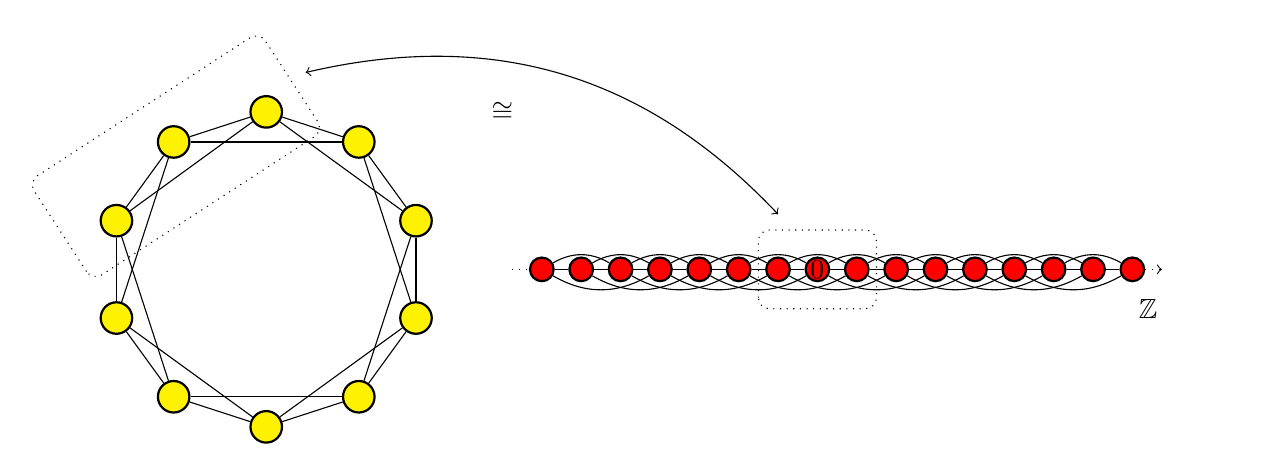
\begin{tikzpicture}[x=1cm,y=1cm]
\node (b1) at (canvas polar cs:angle=90,radius=2cm) [circle, draw=black,thick,fill=yellow,minimum size = 4mm, inner sep = 0]{};
\node (b2) at (canvas polar cs:angle=126,radius=2cm) [circle, draw=black,thick,fill=yellow,minimum size = 4mm, inner sep = 0]{};
\node (b3) at (canvas polar cs:angle=162,radius=2cm) [circle, draw=black,thick,fill=yellow,minimum size = 4mm, inner sep = 0]{};
\node (b4) at (canvas polar cs:angle=198,radius=2cm) [circle, draw=black,thick,fill=yellow,minimum size = 4mm, inner sep = 0]{};
\node (b5) at (canvas polar cs:angle=234,radius=2cm) [circle, draw=black,thick,fill=yellow,minimum size = 4mm, inner sep = 0]{};
\node (b6) at (canvas polar cs:angle=270,radius=2cm) [circle, draw=black,thick,fill=yellow,minimum size = 4mm, inner sep = 0]{};
\node (b7) at (canvas polar cs:angle=306,radius=2cm) [circle, draw=black,thick,fill=yellow,minimum size = 4mm, inner sep = 0]{};
\node (b8) at (canvas polar cs:angle=342,radius=2cm) [circle, draw=black,thick,fill=yellow,minimum size = 4mm, inner sep = 0]{};
\node (b9) at (canvas polar cs:angle=18,radius=2cm) [circle, draw=black,thick,fill=yellow,minimum size = 4mm, inner sep = 0]{};
\node (b10) at (canvas polar cs:angle=54,radius=2cm) [circle, draw=black,thick,fill=yellow,minimum size = 4mm, inner sep = 0]{};
\node (ya1) at (2,0) {};
\node (ya2) at (2.5,0) {};
\node (ya3) at (3.0,0) {};
\node (ya4) at (11.5,0) {};
\node (ya5) at (12,0) {};
\node (ya6) at (12.5,0) {};
\node (c1) at (3.5,0) [circle, draw=black,thick,fill=red,minimum size = 3mm, inner sep = 0]{};
\node (c2) at (4,0) [circle, draw=black,thick,fill=red,minimum size = 3mm, inner sep = 0]{};
\node (c3) at (4.5,0) [circle, draw=black,thick,fill=red,minimum size = 3mm, inner sep = 0]{};
\node (c4) at (5,0) [circle, draw=black,thick,fill=red,minimum size = 3mm, inner sep = 0]{};
\node (c5) at (5.5,0) [circle, draw=black,thick,fill=red,minimum size = 3mm, inner sep = 0]{};
\node (c6) at (6,0) [circle, draw=black,thick,fill=red,minimum size = 3mm, inner sep = 0]{};
\node (c7) at (6.5,0) [circle, draw=black,thick,fill=red,minimum size = 3mm, inner sep = 0]{};
\node (c8) at (7,0) [circle, draw=black,thick,fill=red,minimum size = 3mm, inner sep = 0]{0};
\node (c9) at (7.5,0) [circle, draw=black,thick,fill=red,minimum size = 3mm, inner sep = 0]{};
\node (c10) at (8,0) [circle, draw=black,thick,fill=red,minimum size = 3mm, inner sep = 0]{};
\node (c11) at (8.5,0) [circle, draw=black,thick,fill=red,minimum size = 3mm, inner sep = 0]{};
\node (c12) at (9,0) [circle, draw=black,thick,fill=red,minimum size = 3mm, inner sep = 0]{};
\node (c13) at (9.5,0) [circle, draw=black,thick,fill=red,minimum size = 3mm, inner sep = 0]{};
\node (c14) at (10,0) [circle, draw=black,thick,fill=red,minimum size = 3mm, inner sep = 0]{};
\node (c15) at (10.5,0) [circle, draw=black,thick,fill=red,minimum size = 3mm, inner sep = 0]{};
\node (c16) at (11,0) [circle, draw=black,thick,fill=red,minimum size = 3mm, inner sep = 0]{};
\node (an1) at (11.2,-0.5) {$\Z$};
\foreach \from/\to in 
{b1/b2,b1/b3,b2/b3,b2/b4,b3/b4,b3/b5,b4/b5,b4/b6,b5/b6,b5/b7,b6/b7,b6/b8,b7/b8,b7/b9,b8/b9,b8/b10,b9/b10,b9/b1,b10/b1,b10/b2}
\draw[] (\from) to (\to);
\draw[rounded corners,dotted,rotate around={33:(b2)}] (-3,0.7) rectangle (0.5,2.2);
\draw[rounded corners,dotted] (6.25,-0.5) rectangle (7.75,0.5);
\foreach \from/\to in 
{c1/c2,c2/c3,c3/c4,c4/c5,c5/c6,c6/c7,c7/c8,c8/c9,c9/c10,c10/c11,c11/c12,c12/c13,c13/c14,c14/c15,c15/c16}
\draw[] (\from) to (\to);
\foreach \from/\to in 
{c1/c3,c2/c4,c3/c5,c4/c6,c5/c7,c6/c8,c7/c9,c8/c10,c9/c11,c10/c12,c11/c13,c12/c14,c13/c15,c14/c16}
\draw[bend left] (\from) to (\to);
\foreach \from/\to in 
{c1/c4,c2/c5,c3/c6,c4/c7,c5/c8,c6/c9,c7/c10,c8/c11,c9/c12,c10/c13,c11/c14,c12/c15,c13/c16}
\draw[bend right] (\from) to (\to);
 \draw[dotted] (ya3) -- (c1);
 \draw[dotted, ->] (c16) -- (ya4);
 \draw[bend left, <->] (0.5,2.5) to (6.5,0.7);
 \node at (3,2) {$\cong$};
\end{tikzpicture}

\end{document}